\section{Model and main results}\label{sec:model}
There are communities $C_0=L_0\cup R_0$ and $C_1=L_1\cup R_1$, each side of size $m$, and $q=2m$. At each arrival choose an internal edge in $C_s$ with probability $(1-\eps)/2$, for each $s$, or direction $L_0$--$R_1$ or $L_1$--$R_0$ with probability $\eps/2$ each. Internal edges are uniform on $K_{m,m}$. In cross direction $d$, a fixed nonnegative matrix $B^{(d)}$ has all row and column sums one; conditional edge probability is $B^{(d)}_{ij}/m$. Product sampling has $B=J/m$ and a matching is a permutation matrix. Matrices may depend deterministically on $q$. A randomly selected matrix is admissible if chosen independently before the arrivals, by conditioning on it. Matrices selected from current loads are excluded.

Loads $A_v(n)$ are nonnegative integers, initially zero. Increment the endpoint of smaller load, breaking every tie to the left side. Let
\[
 M_s(n)=\sum_{v\in C_s}A_v(n),\quad \Delta_n=M_0(n)-M_1(n),
 \quad Z_c(n)=\sum_v(A_v(n)-c)_+.
\]
For integer $c$, $Z_c$ is also the number of overflows when each bucket stores its first $c$ assigned items. Indeed the capped loads remain $\min(A_v,c)$ under the same candidate stream: below capacity both comparisons agree, and once both candidates are full the uncapped winner is irrelevant to the overflow count. This identifies the overflow count with the positive-part load functional.

For a pair of integer laws $z=(p_L,p_R)$ with finite first moments, write
\[
 x_k=p_L([k,\infty)),\quad y_k=p_R([k,\infty)),\quad
 a_k=x_k-x_{k+1},\quad b_k=y_k-y_{k+1},
\]
and $\mu(z)=(\E L+\E R)/2$. The metric $d_1$ is the sum of the two marginal Wasserstein distances, equivalently the sum of absolute tail differences. Integer shift $\sh_j$ adds $j$ to both laws.


There are three time scales. After $k$ internal arrivals in one community,
its mean clock is $u=k/q$. The common mean at global arrival $n$ is
$h_n=n/(2q)$. The slow diffusion clock is $t=n/q^2$.
At critical fill $n_*=2qc=4mc$, these give $h_{n_*}=c$ and
$n_*/q^2=c/m\to\kappa$. An offset of $2hq$ arrivals changes the common mean
by $h$ while changing slow time by only $2h/q$.
Figure~\ref{fig:model} shows the candidate structure and the two retained states.

\begin{figure}[t]
\centering
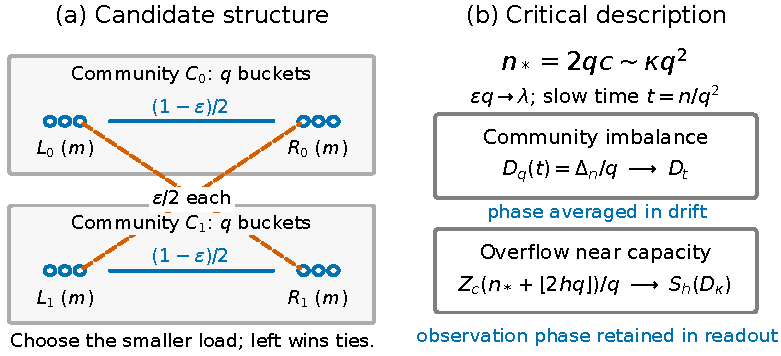
\includegraphics[width=\textwidth]{figures/model_scales.pdf}
\caption{The fixed allocation rule and its critical scales. Each of the four
sides contains $m=q/2$ buckets. Internal directions have probability
$(1-\eps)/2$ each; cross directions have probability $\eps/2$ each.
The offered cross endpoints have uniform marginals under any fixed doubly
stochastic kernel. The algorithm increments the smaller endpoint load and
chooses the left endpoint at a tie. The limiting diffusion retains community
imbalance; the overflow readout also retains the internal profile.}
\label{fig:model}
\end{figure}


For integer capacities $c_q$, set
\[
 n_*=2qc_q,\qquad n_q(h)=n_*+\lfloor2qh\rfloor.
\]
When $c_q/m\to\kappa>0$, each bounded $h$ window has nonnegative indices for large $q$.
The imbalance path $D_q$ linearly interpolates $\Delta_n/q$ at times $n/q^2$.
The overflow curve $F_q$ linearly interpolates $Z_{c_q}(k)/q$ at coordinates
$h=(k-n_*)/(2q)$. Its distance from $Z_{c_q}(n_q(h))/q$ is at most $1/q$.

All path and curve Wasserstein distances below have order one. They use the uniform norm on the corresponding continuous-function space. Joint convergence uses the sum of the path and curve uniform norms. Thus, for a metric $d$, the transport distance is $\inf\E d(U,V)$ over couplings with the stated laws.

\Needspace{10\baselineskip}
\begin{theorem}[Fixed-kernel universality]\label{thm:universal}
For empty starts and fixed $T,\Lambda<\infty$, assume $q\ge4$, $\eps\le1/4$ and $\eps q\le\Lambda$. A genuine fixed-kernel process and a genuine product process admit a coupling such that, for $\mathcal D_n$ the sum of absolute differences of their four separately sorted side vectors,
\[
 \E\max_{n\le Tq^2}\frac{\mathcal D_n}{q}
 =O_{T,\Lambda}(q^{-1/6}\log^2q)\longrightarrow0.
\]
The same bound controls $|\Delta^F-\Delta^P|/q$ and $|Z_c^F-Z_c^P|/q$, simultaneously for all common capacities $c\ge0$.
\end{theorem}

\Needspace{12\baselineskip}
\begin{theorem}[Internal periodic profile]\label{thm:profile}
The mean-clock tail flow
\begin{equation}\label{eq:flow}
 \dot x_k=2a_{k-1}y_{k-1},\qquad
 \dot y_k=2b_{k-1}x_k
\end{equation}
has a unique finite-first-moment periodic family $\rho^u=(L_u,R_u)$ with mean $u$, satisfying
\[
 \rho^{u+1}=\sh_1\rho^u,\qquad \Phi_t\rho^u=\rho^{u+t}.
\]
It has exponential moments, full support at every integer, and
$d_1(\rho^u,\rho^v)=2|u-v|$. Attraction is uniform over centered exponential-moment sublevels and all initial phases. No effective attraction rate is asserted.
\end{theorem}

Define independent-draw comparisons and the overflow readout by
\begin{align}
 H(u,v)&=\Prob(L_u\le R_v),\nonumber\\
 g(h,d)&=H(h+d/2,h-d/2)-H(h-d/2,h+d/2),\label{eq:g}\\
 \gb(d)&=\int_0^1g(h,d)\dd h,\nonumber\\
 \sigma(u)&=\tfrac12\{\E(L_u)_++\E(R_u)_+\},\quad
 S_h(d)=\sigma(h+d/2)+\sigma(h-d/2).\label{eq:spill}
\end{align}

\Needspace{19\baselineskip}
\begin{theorem}[Common critical limit]\label{thm:limit}
If $\eps q\to\lambda\in[0,\infty)$, then for every fixed $T$, $D_q\to D$ in first Wasserstein distance for the uniform path norm on $[0,T]$, where
\begin{equation}\label{eq:sde}
 \dd D_t=\dd B_t+\lambda\gb(D_t)\dd t,\qquad D_0=0.
\end{equation}
The function $\gb$ is odd, smooth, strictly decreasing, globally $2$-Lipschitz and negative on $(0,\infty)$, with $\gb'(0)<0$ and $\gb(d)\to-\operatorname{sign}(d)$ at infinity. Let the integer capacities satisfy $c_q/m\to\kappa\in(0,\infty)$. For each $H_0<\infty$ and $T_*>\kappa$,
\[
 \bigl(D_q|_{[0,T_*]},F_q|_{[-H_0,H_0]}\bigr)
 \longrightarrow
 \bigl(D|_{[0,T_*]},(S_h(D_\kappa))_{|h|\le H_0}\bigr)
\]
in first Wasserstein distance for the sum of the two uniform norms. Restriction gives joint convergence with any shorter path horizon. This holds for every fixed kernel above. The function $S_h$ is even and convex in $d$, $1$-Lipschitz in $d$, and $2$-Lipschitz in $h$, with $S_0(0)>0$.
\end{theorem}

The drift averages the common phase along many complete cycles. The overflow
readout at the integer critical count has phase zero and is not phase averaged.
The function $S_h$ is not periodic in $h$: the observation offset changes the
fill level as well as the lattice phase. Theorem~\ref{thm:universal} gives an
explicit but conservative kernel-comparison bound. The joint critical limit
has no effective uniform finite-size error bound.

Figure~\ref{fig:mechanism} displays the profile and averaged response.

\begin{figure}[t]
\centering
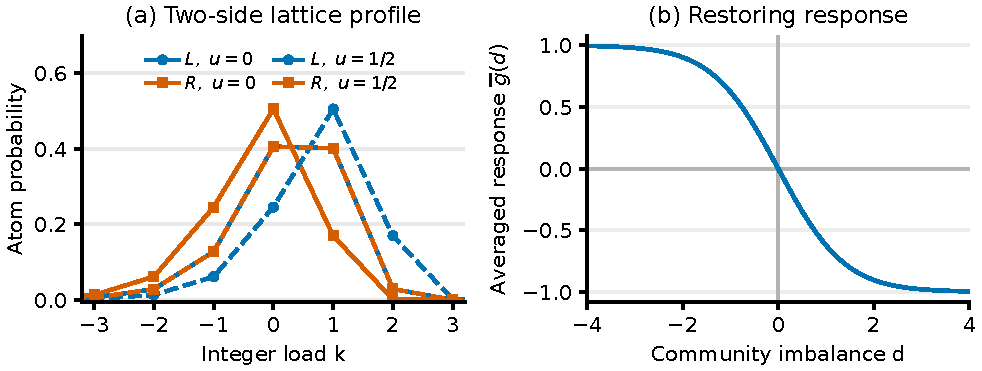
\includegraphics[width=\textwidth]{figures/profile_mechanism.pdf}
\caption{Internal structure and restoring response, replotted from saved
profile nodes and the frozen response table. Left: left and right atom
probabilities at mean phases $u=0$ (solid) and $u=1/2$ (dashed).
Only the displayed load levels are shown. The half-phase operation swaps
the sides and shifts the new left law by one. Right: the phase-averaged
response $\gb(d)$; positive imbalance has negative response.
Connecting segments are for display. No new trajectory or numerical solution
enters this figure.}
\label{fig:mechanism}
\end{figure}

\begin{corollary}[A leading internal overflow contribution]\label{cor:internalexcess}
Under Theorem~\ref{thm:limit}, fix $\kappa>0$ and $\lambda<\infty$. Let $X_u$ have the equal mixture of the two laws in $\rho^u$, and set
\[
 r(u)=\E(X_u)_+-u_+=\tfrac12(\E|X_u|-|u|).
\]
Then $r(u)>0$ for every finite $u$, and
\[
 S_0(d)=\frac{|d|}{2}+r(d/2)+r(-d/2).
\]
For every admissible fixed cross kernel,
\[
 \lim_{q\to\infty}\E\left[\frac{Z_{c_q}(n_*)-|\Delta_{n_*}|/2}{q}\right]
 =\E\{r(D_\kappa/2)+r(-D_\kappa/2)\}>0.
\]
The positive limit may depend on $\kappa$ and $\lambda$.
\end{corollary}
\begin{proof}
The mixture has mean $u$. Full support from Theorem~\ref{thm:profile} gives positive mass on both sides of zero. Hence $\E|X_u|>|\E X_u|=|u|$. Substitution into \eqref{eq:spill} gives the displayed decomposition.

At $n_*=2qc_q$, the community excess totals are $\Delta_{n_*}/2$ and $-\Delta_{n_*}/2$. Taking positive parts within each community yields the exact finite-size inequality $Z_{c_q}(n_*)\ge|\Delta_{n_*}|/2$. Put $\kappa_q=n_*/q^2\to\kappa$. The endpoint-time estimate \eqref{eq:endpointtime} shows $\E|D_q(\kappa_q)-D_q(\kappa)|\to0$. The joint first Wasserstein convergence in Theorem~\ref{thm:limit} therefore passes expectations for the Lipschitz, linear-growth difference readout. This gives the stated limit. Its integrand is strictly positive at every finite value of $D_\kappa$, and its expectation is finite.
\end{proof}

This corollary identifies the information omitted by an imbalance-only approximation. It follows from the profile and critical-limit theorems. It does not assert a uniform positive gap over all parameters. The imbalance-only readout is a mechanistic simplification, rather than a claimed strongest published competitor.

\begin{corollary}[Capacity consequences]\label{cor:capacity}
Under Theorem~\ref{thm:limit}, let $s_*=S_0(0)>0$ and
$C_{\kappa,\lambda}=\E S_0(D_\kappa)$. For each fixed $a\in(0,s_*)$,
\[
 \Prob\{Z_{c_q}(n_*)\ge aq\}\longrightarrow1,
 \qquad \Prob\{Z_{c_q}(n_*)=0\}\longrightarrow0.
\]
Moreover,
\[
 \E Z_{c_q}(n_*)=qC_{\kappa,\lambda}+o(q),\qquad
 \frac{\E Z_{c_q}(n_*)}{n_*}
 =\frac{C_{\kappa,\lambda}}{\kappa q}+o(q^{-1}).
\]
These conclusions and their leading coefficient hold for every admissible
fixed cross kernel.
\end{corollary}
\begin{proof}
Evenness and convexity give $S_0(d)\ge S_0(0)>a$ for every $d$.
Weak convergence of $Z_{c_q}(n_*)/q$ and the open-set inequality therefore give
the probability limits. First Wasserstein convergence passes its expectation
to $C_{\kappa,\lambda}<\infty$. Finally, $n_*/q^2\to\kappa>0$ gives the
fractional asymptotic. The common limit is independent of the fixed cross kernel.
\end{proof}

Kernel choice within the stated class does not remove the leading overflow
cost. This consequence of the joint law does not compare other allocation strategies.
